\subsection{Covector Definition:}

Covectors and vectors are fundamentally different objects\footnote{Covectors can
"basically" be regarded as row vectors. However, only in an orthormal basis there is a
trivial link to column vector components. This is not true in the general case of
non-orthonormal basis vectors.}. Covectors are functions that take vectors as arguments.
They yield a scalar output $\alpha$ on a vector input $\vec{v}$:

\begin{equation}
    \alpha(\vec{v}) = \alpha_1 v^1 + \alpha_2 v^2 + \dots + \alpha_n v^n =
    \sum\limits_{i}\alpha_i \hdvc{i} 
\end{equation}

Covectors take an input from vector space $V$ and return a real number $\alpha$, i.e.
$\alpha: V \rightarrow \mathbb{R}$. Covectors have the linearity properties, i.e. they are
linear functions:

\begin{equation}
    \label{eq:covector_linearity}
    \begin{array}{rcl}
        \alpha(\textcolor{ForestGreen}{\vec{v}}+\textcolor{RoyalPurple}{\vec{w}}) & = &
        \alpha(\textcolor{ForestGreen}{\vec{v}})+\alpha(\textcolor{RoyalPurple}{\vec{w}}) \\
        \alpha(\textcolor{Goldenrod}{n}\textcolor{ForestGreen}{\vec{v}}) & = &
        \textcolor{Goldenrod}{n}\alpha(\textcolor{ForestGreen}{\vec{v}}) \\
        \alpha(\textcolor{Goldenrod}{n}\textcolor{ForestGreen}{\vec{v}}+
        \textcolor{YellowOrange}{m}\textcolor{RoyalPurple}{\vec{w}}) & = &
        \textcolor{Goldenrod}{n}\alpha(\textcolor{ForestGreen}{\vec{v}})+
        \textcolor{YellowOrange}{m}\alpha(\textcolor{RoyalPurple}{\vec{w}})
    \end{array}
\end{equation}

Covectors can also be viewed as elements of their own vector space $V^*$, i.e. they can be
scaled and added:

\begin{equation}
    \label{eq:covector_add_scale}
    \begin{array}{rcl}
        (n\alpha)(\hdv) & = &
        n\alpha(\hdv)\\
        (\beta + \gamma)(\hdv) & = &
        \beta(\hdv)+ \gamma(\hdv)
    \end{array}
\end{equation}

The vector space of contravariant vectors is defined by $(V,S,+,\cdot)$. The vector space
of covectors is defined by $(V^*,S,\textcolor{red}{+},\textcolor{red}{\cdot})$. The
covector operations $\textcolor{red}{+}$ and $\textcolor{red}{\cdot}$ are different from
the corresponding $+$ and $\cdot$ operations of vectors.

Covectors can be visualized as oriented stacks of lines of constant function value. When
the coordinates are vizualized as vectors they would provide a vector oriented as the
normal to the stack height lines:
\begin{figure}[h]
    \centering
    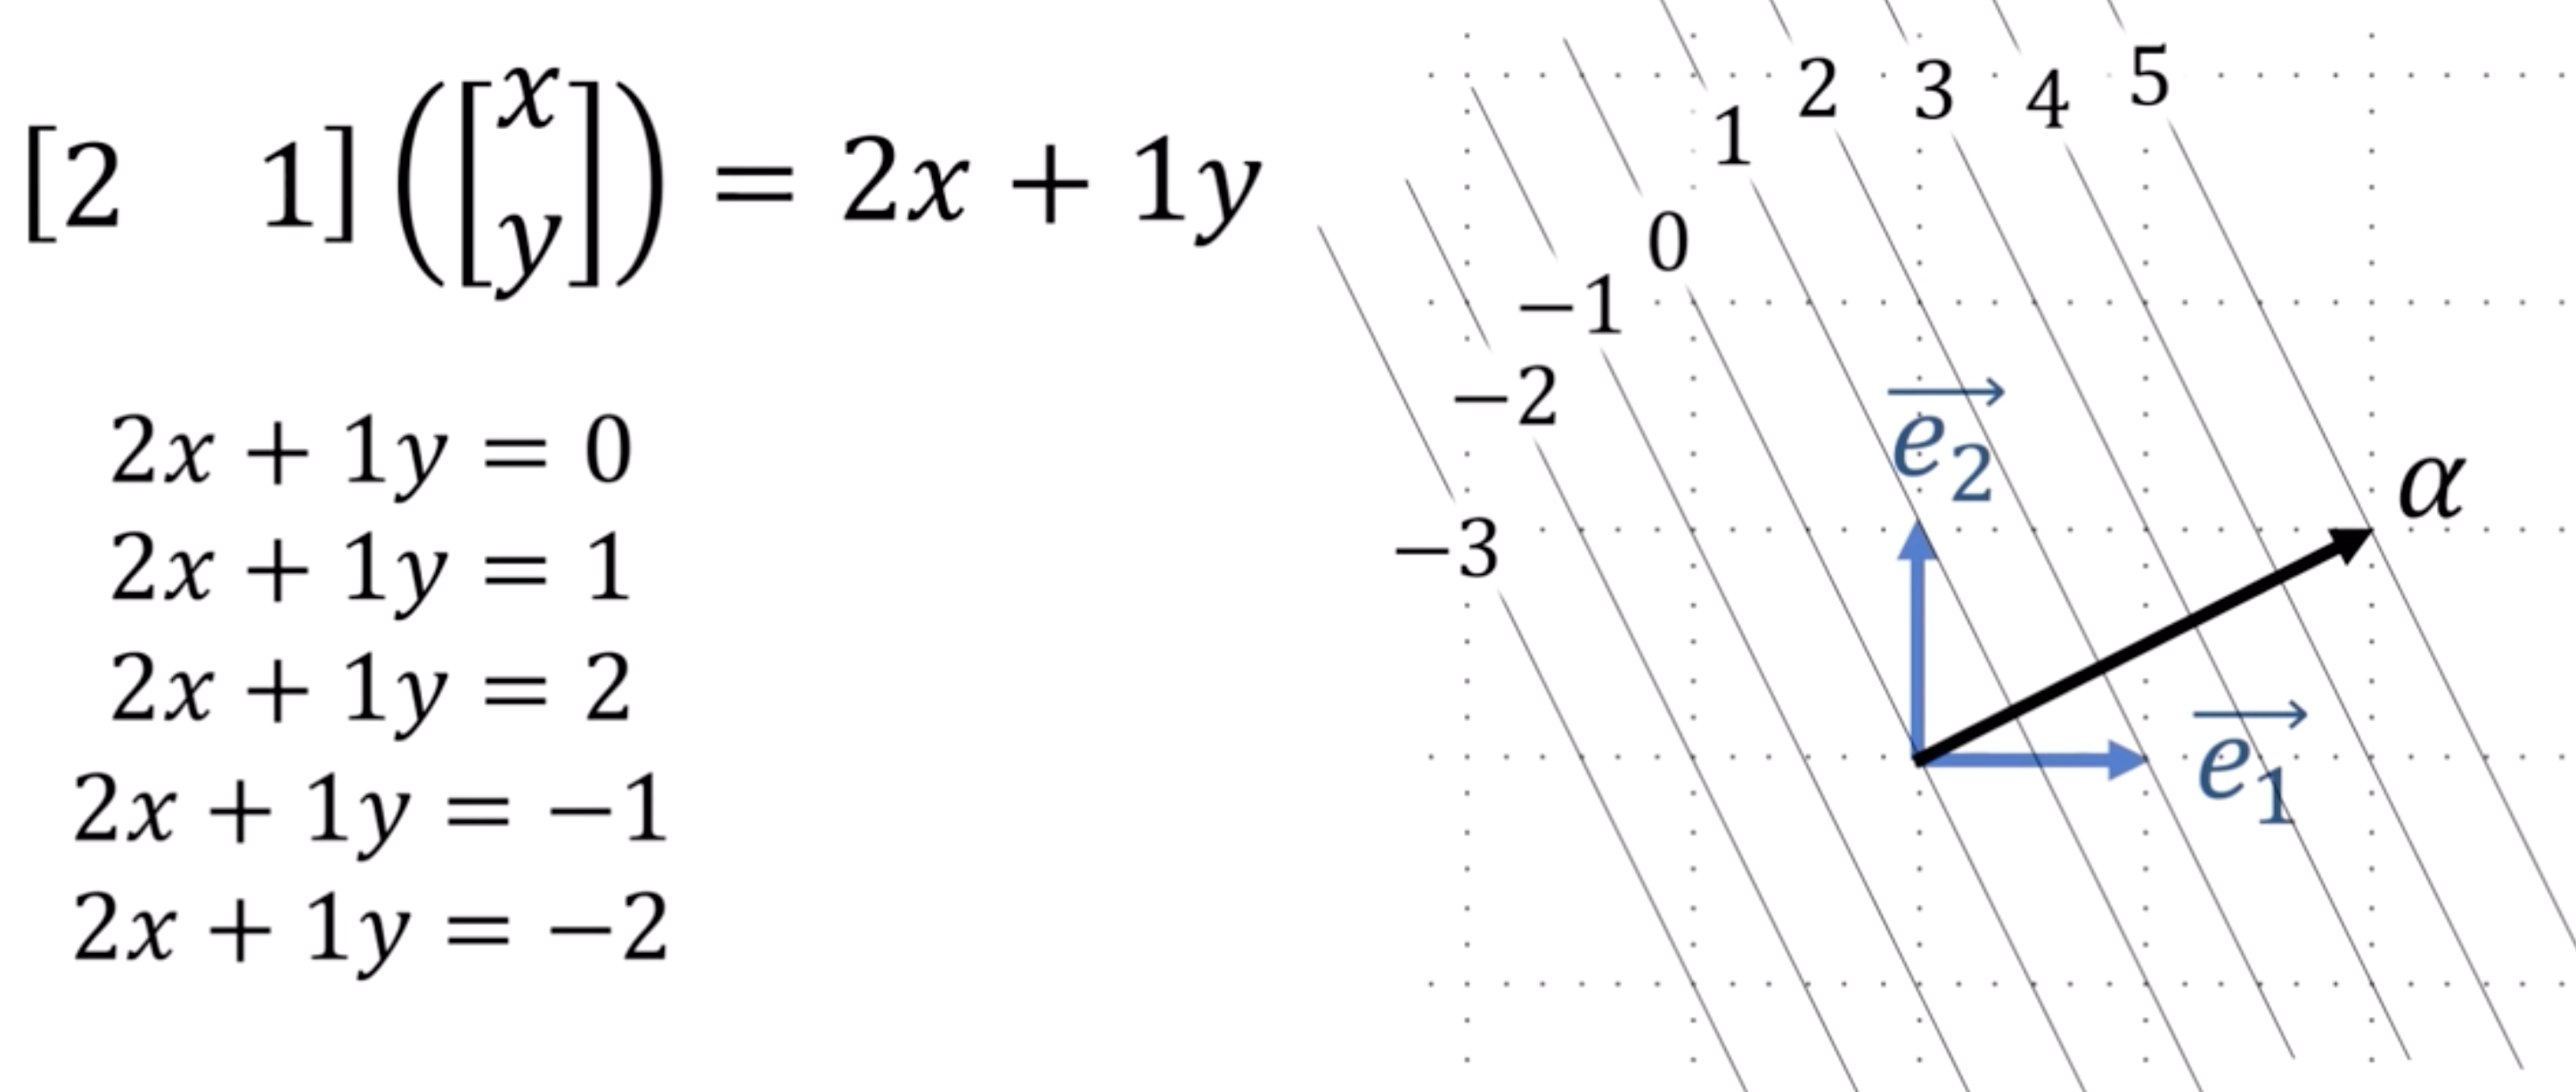
\includegraphics[width=0.7\textwidth]{Covector_as_oriented_stack_eigenchris}
    \caption{Example: covector visualized as lines of constant function value}
    \label{fig:covector_visualized}
\end{figure}

The function values returned by the covector can be visualized depending on the vectors
provided as arguments. The number of height lines pierced by the vector gives the returned
result:
\begin{figure}[h]
    \centering
    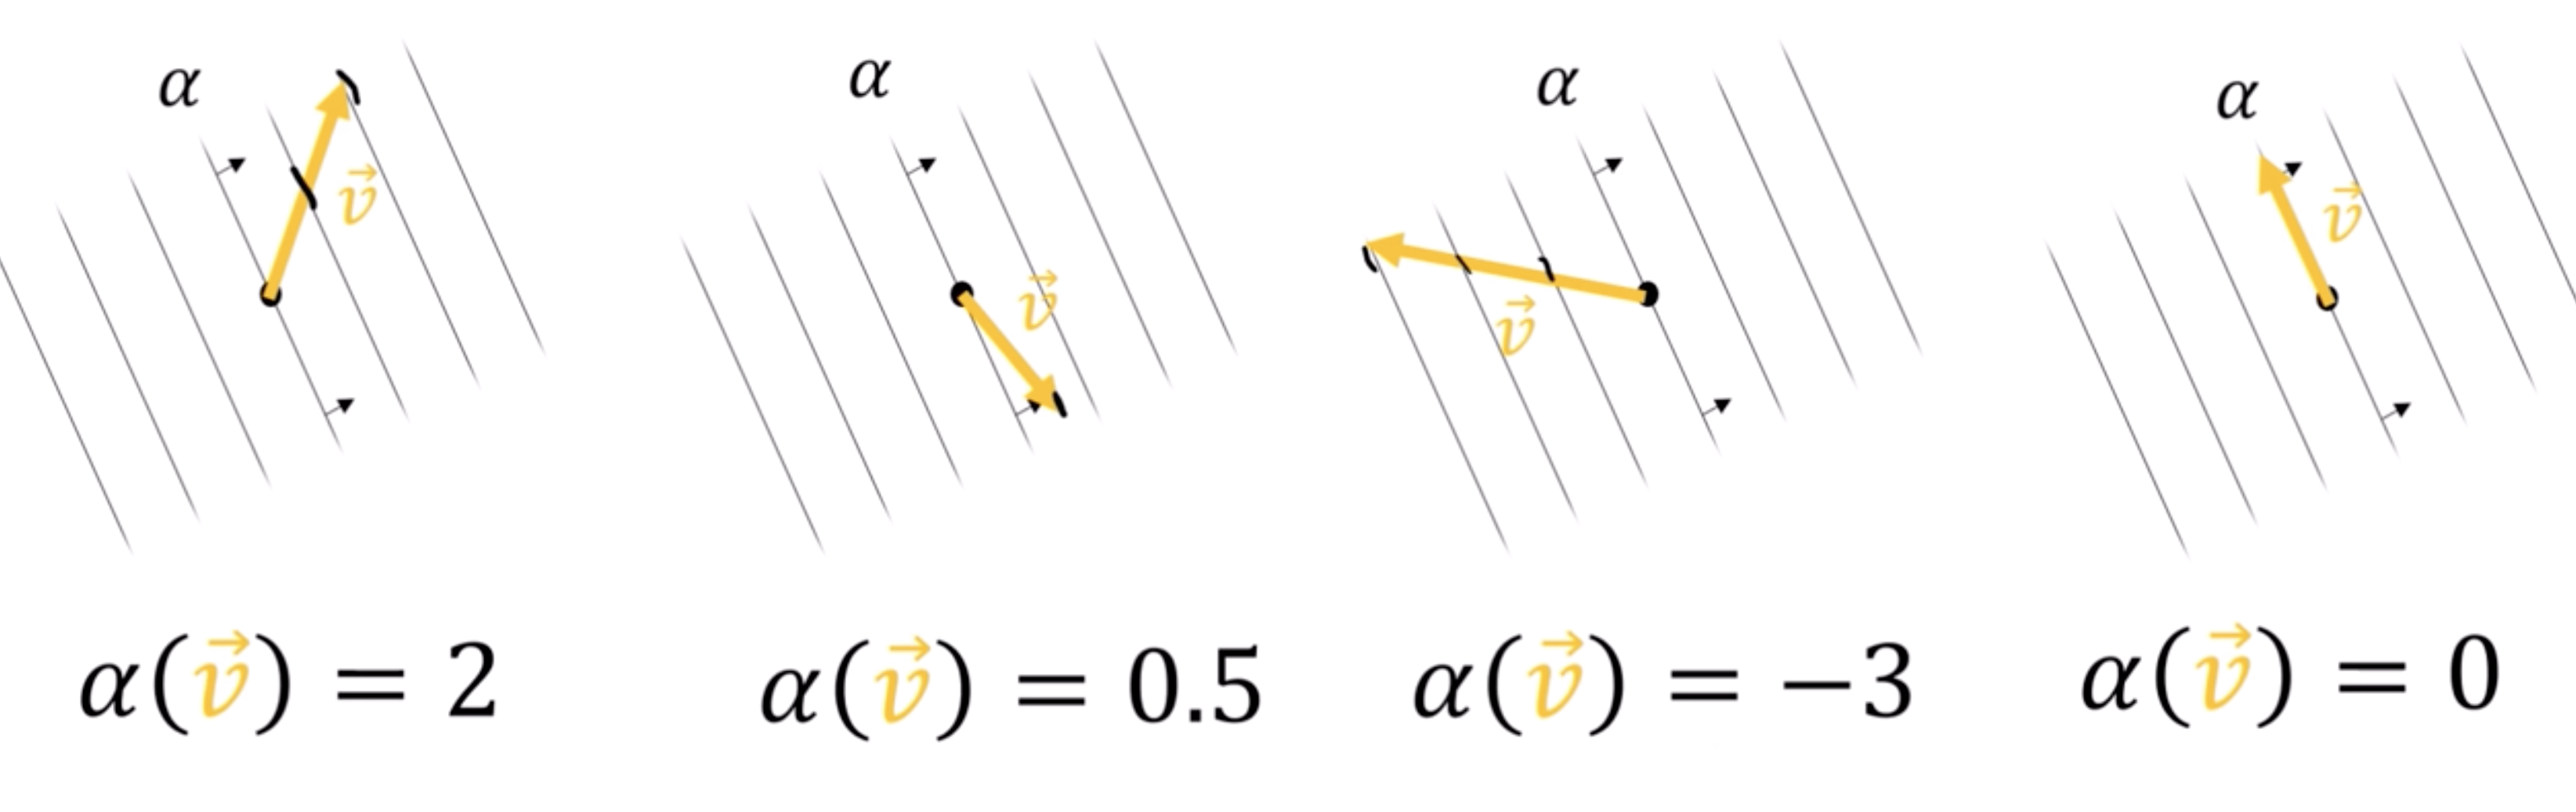
\includegraphics[width=0.9\textwidth]{Covector_return_values_eigenchris}
    \caption{Example: covector return values from given input vectors}
    \label{fig:covector_return_values}
\end{figure}

\begin{itemize}
    \item Covectors are \textcolor{red}{invariant} under a change of the coordinate
    system.
    \item Covector components are \textcolor{red}{not invariant} under a change of the
    coordinate system.
\end{itemize}

Covectors are functions $\alpha: V \rightarrow \mathbb{R}$ that take vectors as arguments.
Covectors don't live in the vector space $V$, but in $V^*$. Thus we cannot use basis
vectors like \{\hdbv{1}, \hdbv{2}\} to measure covectors directly. But still the basis
\{\hdbv{1}, \hdbv{2}\} can be used to derive a special covector basis \{\hdcbvc{1},
\hdcbvc{2}\} with the specific property:

\begin{equation}
    \label{eq:covec_vec_link}
    \begin{array}{rcl}
        \hdcbvc{i}(\hdbv{j}) & = &
        \delta^i_j = 
        \begin{cases}
            1, & \text{if}\ i = j \\
            0, & \text{if}\ i \neq j
        \end{cases} \\
        \noalign{\vskip10pt}
        \text{such that for the 2D case:}\qquad
        \hdcbvc{1}(\hdbv{1}) & = & 1 \qquad\qquad
        \hdcbvc{1}(\hdbv{2}) = 0 \\
        \hdcbvc{2}(\hdbv{1}) & = & 0 \qquad\qquad
        \hdcbvc{2}(\hdbv{2}) = 1
    \end{array}
\end{equation}

This effectively links the bases \hdcbvc{i} and \hdbv{i} and the vector spaces $V$ and
$V^*$, making $V^*$ the dual space of $V$. It enables us to use these covectors to find
the coordinates of arbitrary vectors of $V$ by applying these special covectors to them:

\begin{equation}
    \begin{array}{rcl}
        \label{eq:covec_application}
        \hdcbvc{1}(\hdv) & = &
        \hdcbvc{1}(\hdvc{1}\hdbv{1} + \hdvc{2}\hdbv{2})
        \underset{(\ref{eq:covector_linearity})}{=}
        \hdvc{1}\hdcbvc{1}(\hdbv{1}) + \hdvc{2}\hdcbvc{1}(\hdbv{2})
        \underset{(\ref{eq:covec_vec_link})}{=}
        \hdvc{1} \\
        \hdcbvc{2}(\hdv) & = &
        \hdcbvc{2}(\hdvc{1}\hdbv{1} + \hdvc{2}\hdbv{2})
        \underset{(\ref{eq:covector_linearity})}{=}
        \hdvc{1}\hdcbvc{2}(\hdbv{1}) + \hdvc{2}\hdcbvc{2}(\hdbv{2})
        \underset{(\ref{eq:covec_vec_link})}{=}
        \hdvc{2} \\
        \noalign{\vskip10pt}
        \Rightarrow \hdcbvc{i}(\hdv) & = & \hdvc{i}
    \end{array}
\end{equation}

This means we select a special covector basis that is aligned with our vector basis such
that each covector basis selects it's corresponding basis vector contribution exclusively:
\\

\begin{figure}[h]
    \centering
    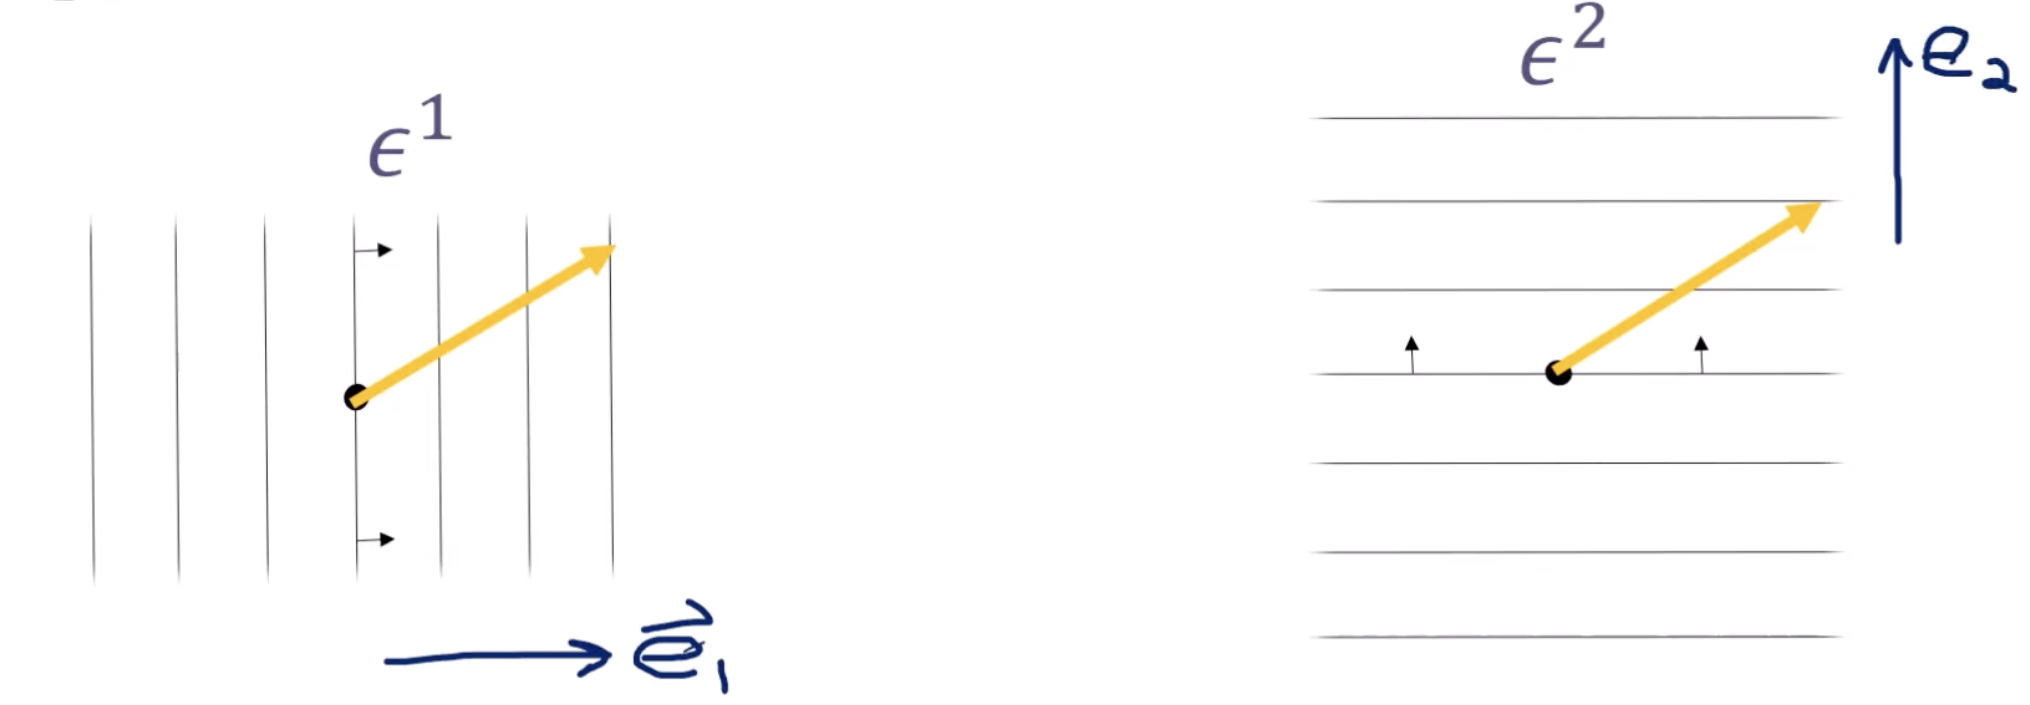
\includegraphics[width=0.8\textwidth]{Special_covector_bases_eigenchris}
    \caption{Example: specifically chosen covector basis}
    \label{fig:selected_covector_basis}
\end{figure}

If we now want to apply a general covector $\alpha$ to a vector $\hdv$ we can transform
the equations by defining the covector components in terms of our specially chosen
covector basis vectors \hdcbvc{1} and \hdcbvc{2}:

\begin{equation}
    \label{eq:covector_with_respect_to_old_basis} 
    \begin{array}{rcl}
        \alpha(\hdv) & = &
        \alpha(\hdvc{1}\hdbv{1} + \hdvc{2}\hdbv{2})
        \underset{(\ref{eq:covector_linearity})}{=}
        \hdvc{1}\alpha(\hdbv{1}) + \hdvc{2}\alpha(\hdbv{2}) \\
        & \underset{(\ref{eq:covec_application})}{=} &
        \hdcbvc{1}(\hdv)\alpha(\hdbv{1}) + \hdcbvc{2}(\hdv)\alpha(\hdbv{2}) \\
        \noalign{\vskip10pt}
        \text{defining}:\ \alpha(\hdbv{1}) & = & \alpha_1 \\
        \alpha(\hdbv{2}) & = & \alpha_2\\ 
        \noalign{\vskip10pt}
        \alpha(\hdv) & = &
        \alpha_1\hdcbvc{1}(\hdv) + \alpha_2\hdcbvc{2}(\hdv) \\
        & \underset{(\ref{eq:covector_add_scale})}{=} &
        (\alpha_1\hdcbvc{1} + \alpha_2\hdcbvc{2})(\hdv) \\
        \noalign{\vskip10pt}
        \Rightarrow \alpha & = & \alpha_1\hdcbvc{1} + \alpha_2\hdcbvc{2}
        = \alpha_i \hdcbvc{i}
    \end{array}
\end{equation}

Thus every covector can be expressed as a linear combination of our specifically chosen
covector basis. We call the basis \{\hdcbvc{1}, \hdcbvc{2}\} the ``dual basis'' of the vector
space $V^*$. Fig.~\ref{fig:arbitrary_covector_linearcombination} shows this graphically.\\

\begin{figure}[h]
    \centering
    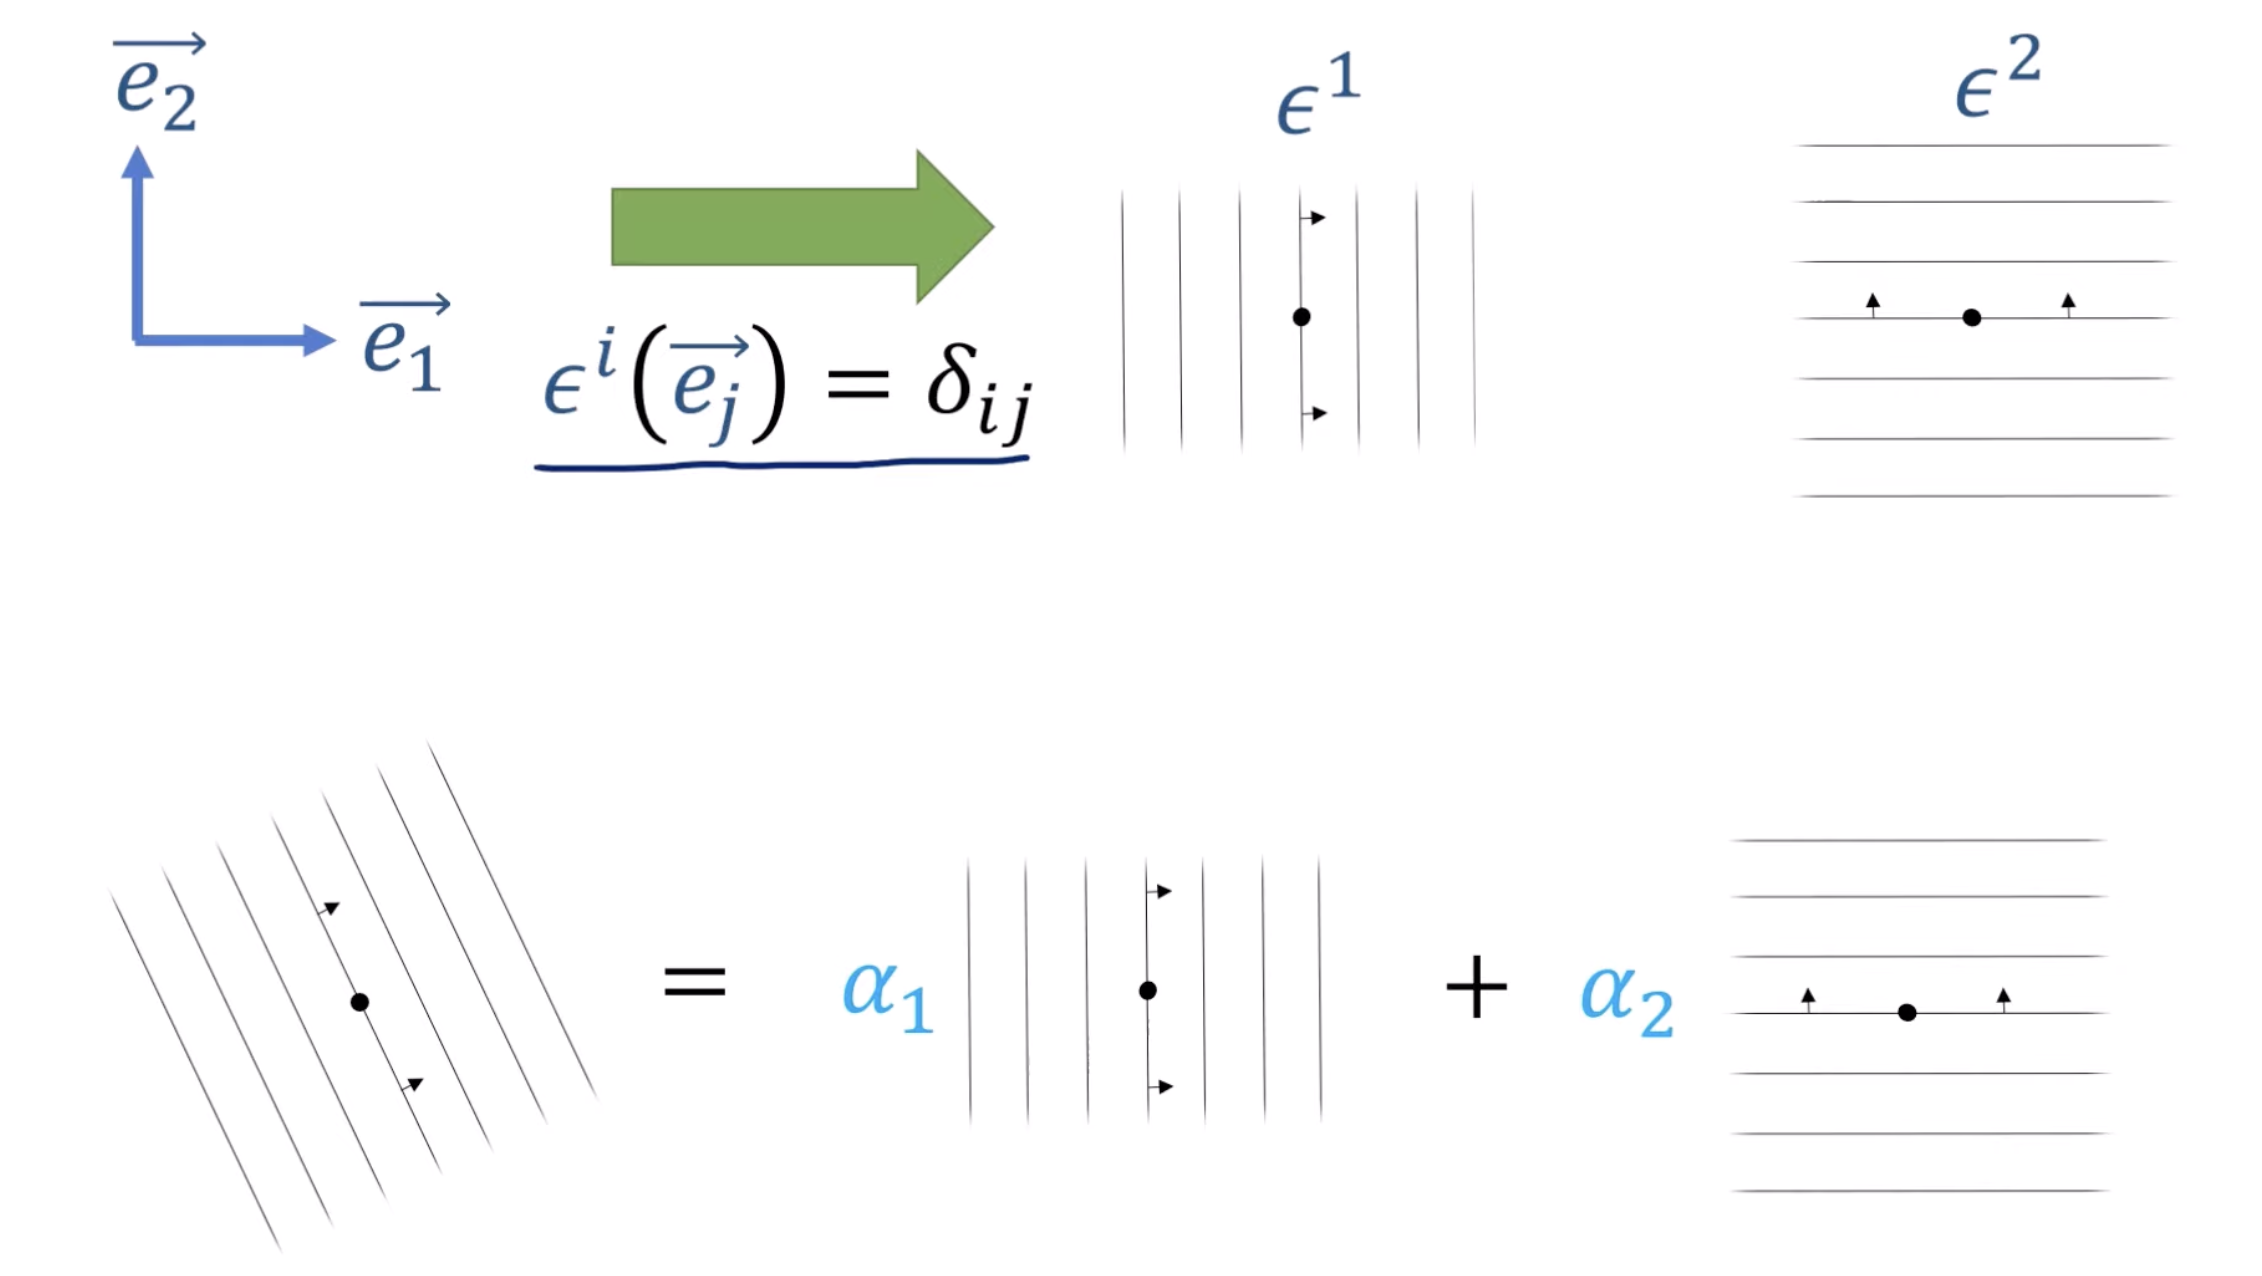
\includegraphics[width=0.6\textwidth]{Arbitray_covector_as_linearcombination_eigenchris}
    \caption{Arbitrary covector (lower row left) expressed as linear combination of the
    covector basis \{\hdcbvc{1}, \hdcbvc{2}\} after the dual basis has been derived from
    the vector basis.}
    \label{fig:arbitrary_covector_linearcombination}
\end{figure}

Of course we could also define an arbitray covector with respect to the vector basis in
the new system: The basis \{\hdbtv{1}, \hdbtv{2}\} can be used to derive a special
covector basis \{\hdcbtvc{1}, \hdcbtvc{2}\} with the specific property:
\begin{equation}
    \label{eq:covec_vec_link_new}
    \begin{array}{rcl}
        \hdcbtvc{i}(\hdbtv{j}) & = &
        \delta^i_j = 
        \begin{cases}
            1, & \text{if}\ i = j \\
            0, & \text{if}\ i \neq j
        \end{cases} \\
        \noalign{\vskip10pt}
        \text{such that for the 2D case:}\qquad
        \hdcbtvc{1}(\hdbtv{1}) & = & 1 \qquad\qquad
        \hdcbtvc{1}(\hdbtv{2}) = 0 \\
        \hdcbtvc{2}(\hdbtv{1}) & = & 0 \qquad\qquad
        \hdcbtvc{2}(\hdbtv{2}) = 1
    \end{array}
\end{equation}

This effectively links the bases \hdcbtvc{i} and \hdbtv{i} and the vector spaces $V$ and
$V^*$, making $V^*$ the dual space of $V$. It enables us to use these covectors to find
the coordinates of arbitrary vectors of $V$ by applying these special covectors to them:

\begin{equation}
    \begin{array}{rcl}
        \label{eq:covec_application_new}
        \hdcbtvc{1}(\hdv) & = &
        \hdcbtvc{1}(\hdtvc{1}\hdbtv{1} + \hdtvc{2}\hdbtv{2})
        \underset{(\ref{eq:covector_linearity})}{=}
        \hdtvc{1}\hdcbtvc{1}(\hdbtv{1}) + \hdtvc{2}\hdcbtvc{1}(\hdbtv{2})
        \underset{(\ref{eq:covec_vec_link_new})}{=}
        \hdtvc{1} \\
        \hdcbtvc{2}(\hdv) & = &
        \hdcbtvc{2}(\hdtvc{1}\hdbtv{1} + \hdtvc{2}\hdbtv{2})
        \underset{(\ref{eq:covector_linearity})}{=}
        \hdtvc{1}\hdcbtvc{2}(\hdbtv{1}) + \hdtvc{2}\hdcbtvc{2}(\hdbtv{2})
        \underset{(\ref{eq:covec_vec_link_new})}{=}
        \hdtvc{2} \\
        \noalign{\vskip10pt}
        \Rightarrow \hdcbtvc{i}(\hdv) & = & \hdtvc{i}
    \end{array}
\end{equation}

This leads to another dual basis specific for the basis vectors in the new
system as shown in equation~\ref{eq:covector_with_respect_to_new_basis}.

\begin{equation}
    \label{eq:covector_with_respect_to_new_basis} 
    \begin{array}{rcl}
        \alpha(\hdv) & = &
        \alpha(\hdtvc{1}\hdbtv{1} + \hdtvc{2}\hdbtv{2})
        \underset{(\ref{eq:covector_linearity})}{=}
        \hdtvc{1}\alpha(\hdbtv{1}) + \hdtvc{2}\alpha(\hdbtv{2}) \\
        & \underset{(\ref{eq:covec_application_new})}{=} &
        \hdcbtvc{1}(\hdv)\alpha(\hdbtv{1}) + \hdcbtvc{2}(\hdv)\alpha(\hdbtv{2}) \\
        \noalign{\vskip10pt}
        \text{defining:}\ \alpha(\hdbtv{1}) & = & \widetilde{\alpha_1} \\
        \alpha(\hdbtv{2}) & = & \widetilde{\alpha_2} \\ 
        \noalign{\vskip10pt}
        \alpha(\hdv) & = &
        \widetilde{\alpha_1}\hdcbtvc{1}(\hdv) + \widetilde{\alpha_2}\hdcbtvc{2}(\hdv) \\
        & \underset{(\ref{eq:covector_add_scale})}{=} &
        (\widetilde{\alpha_1}\hdcbtvc{1} + \widetilde{\alpha_2}\hdcbtvc{2})(\hdv) \\
        \noalign{\vskip10pt}
        \Rightarrow \alpha & = & \widetilde{\alpha_1}\hdcbtvc{1} + 
        \widetilde{\alpha_2}\hdcbtvc{2} =
        \widetilde{\alpha_i}\hdcbtvc{i}
    \end{array}
\end{equation}


Graphically fig.~\ref{fig:covectors_new_system} shows the covectors with respect to the
basis in the new system.\\

\begin{figure}[h]
    \centering
    \begin{subfigure}[b]{0.5175\textwidth}
        \centering
        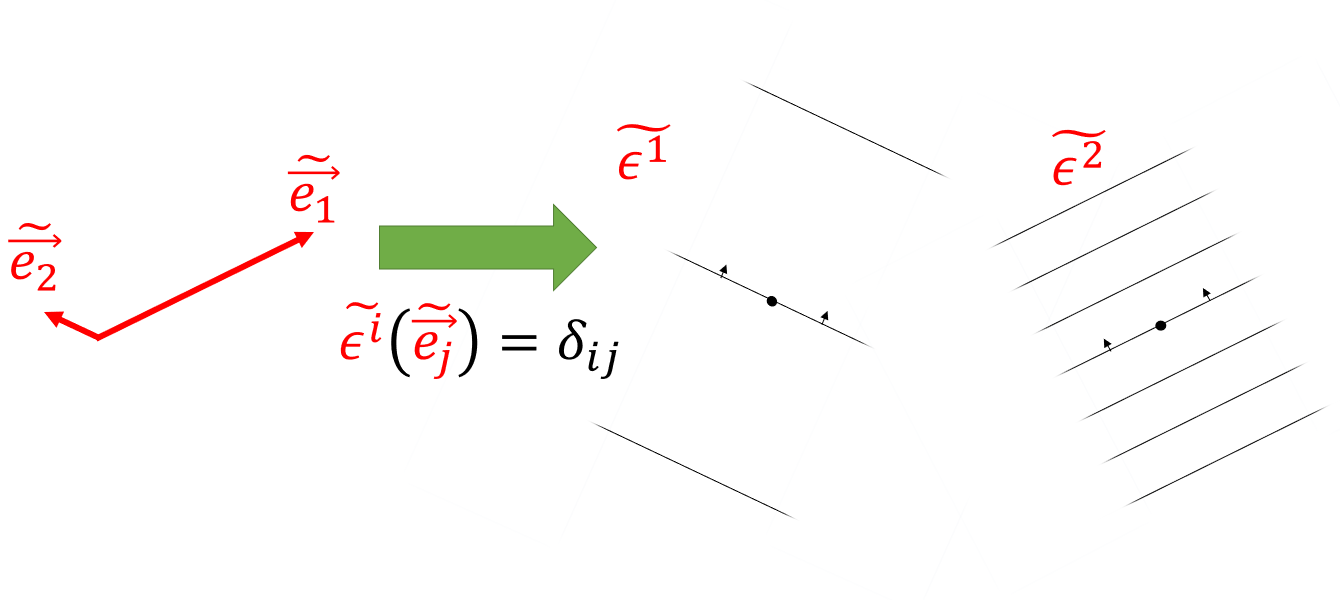
\includegraphics[width=\textwidth]{Covector_eigenchris1}
        \caption{Covector hight lines (new basis)}
    \end{subfigure}
    \hfill
    \begin{subfigure}[b]{0.45\textwidth}
        \centering
        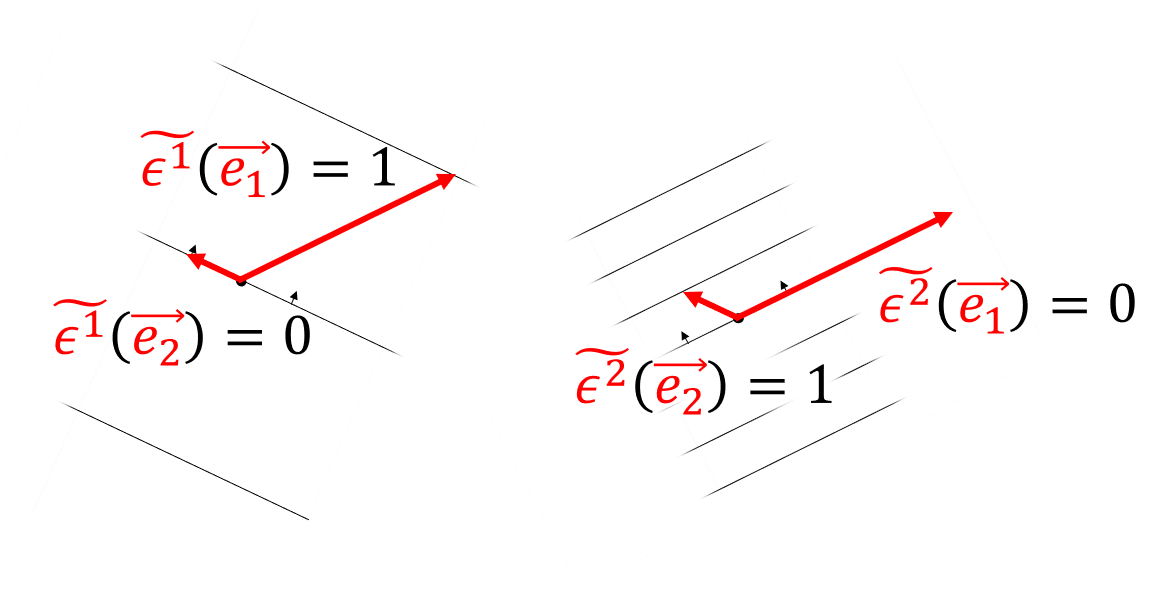
\includegraphics[width=\textwidth]{Covector_eigenchris2}
        \caption{Covector function (new basis)}
    \end{subfigure}
    \caption{Another dual covector basis expressed with respect to the basis in the new
    system}
    \label{fig:covectors_new_system}
\end{figure}

In order to derive the transformation rules for the the covector basis we use
\{\hdcbvc{j}\} as the old basis for $V^*$ and \{\hdcbtvc{i}\} as the new basis for $V^*$.
The new basis can be expressed by a linear combination of the old basis vectors using the
coefficients $Q^{i~}_{~j}$:
\begin{equation}
    \label{eq:covector_new_basis_as_linearcombination_in_old_basis}
    \hdcbtvc{i} = Q^{i~}_{~j}\hdcbvc{j}
\end{equation}

Using~(\ref{eq:covec_vec_link_new}) and
(\ref{eq:covector_new_basis_as_linearcombination_in_old_basis}) we can write:

\begin{equation}
    \label{eq:covector_transformation_rule} 
    \begin{array}{rcl}
        \hdcbtvc{i}(\hdbtv{k}) & = &
        Q^{i~}_{~j}\hdcbvc{j}(\hdbtv{k}) \\
        \delta^i_k &
        \underset{(\ref{eq:covec_vec_link_new}),(\ref{eq:forward_trafo})}{=} &
        Q^{i~}_{~j}\hdcbvc{j}(F^{l~}_{~k}\hdbv{l})
        \underset{(\ref{eq:covector_linearity})}{=}
        Q^{i~}_{~j} F^{l~}_{~k}\hdcbvc{j}(\hdbv{l}) \\
        \delta^i_k &
        \underset{(\ref{eq:covec_vec_link})}{=} &
        Q^{i~}_{~j} F^{l~}_{~k} \delta^j_l = Q^{i~}_{~j} F^{j~}_{~k} \\
        \text{comparing with~(\ref{eq:forward_backward_inverse}):\quad}
        Q^{i~}_{~j} & = & B^{i~}_{~j} \\
        \noalign{\vskip10pt}
        \text{inserting in~(\ref{eq:covector_new_basis_as_linearcombination_in_old_basis})}
        \Rightarrow \hdcbtvc{i} & = & B^{i~}_{~j}\hdcbvc{j}
    \end{array}
\end{equation}

This shows that covectors transform with the backward transformation from the old to the
new basis. Using the same approach it can be shown that:
\begin{equation}
    \label{eq:covector_transformation_rule_new}
    \begin{array}{rcl}
        \Rightarrow \hdcbvc{i} & = & F^{i~}_{~j}\hdcbtvc{j}
    \end{array}
\end{equation}

Summarizing the transformation rules for vectors and covectors we get:
\begin{equation}
    \label{eq:vector_covector_trafo_overview}
    \begin{array}{rclrcl}
      \hdbtvc{j} & = & F^{i~}_{~j}\hdbvc{i}
      \qquad\qquad
      \hdcbtvc{i} & = & B^{i~}_{~j} \hdcbvc{j} \\
      \hdbvc{j} & = & B^{i~}_{~j}\hdbtvc{i}
      \qquad\qquad
      \hdcbvc{i} & = &  F^{i~}_{~j} \hdcbtvc{j}
    \end{array}
  \end{equation}

The covector can be constructed from the basis in the old and new basis:
\begin{equation}
    \label{eq:covector_representation}
    \alpha = \alpha_i\hdcbvc{i} = \widetilde{\alpha_j}\hdcbtvc{j}
\end{equation}
By inserting the transformation rule~(\ref{eq:covector_transformation_rule})
or~(\ref{eq:covector_transformation_rule_new}) and comparing with the other part of the
equation~(\ref{eq:covector_representation}) we can get the transformation rules for the
covector components:
\begin{equation}
    \label{eq:covector_component_trafo}
    \begin{array}{rclrcl}
      \widetilde{\alpha_j} & = & F^{i~}_{~j}\alpha_i \\
      \alpha_j & = & B^{i~}_{~j}\widetilde{\alpha_i}
    \end{array}
  \end{equation}
  This means that covector components transform as the basis vectors do, i.e. with the
  forward transformation from the old to the new system and with the backward
  transformation from the new to the old system. This is called covariant transformation
  behaviour. For both cases the summation goes via the first index of the transformation
  matrix (equivalent to matrix multiplication from the left). \\

  Summing up everything so far we get:
  \begin{equation}
    \label{eq:summary_transformations}
    \boxed{
    \begin{array}{rclrcl}
      \hdbtvc{j} & = & F^{i~}_{~j}\hdbvc{i}
      \qquad \hfill
      \hdcbtvc{i} & = & B^{i~}_{~j} \hdcbvc{j}
      \quad\text{(\underline{contra}var.)} \\
      \hdbvc{j} & = & B^{i~}_{~j}\hdbtvc{i}
      \qquad\hfill
      \hdcbvc{i} & = &  F^{i~}_{~j} \hdcbtvc{j} \hfill \\
      \noalign{\vskip10pt}
      \text{with:}\quad \hdv & = & \hdvc{i} \hdbvc{i} = \hdtvc{j} \hdbtvc{j}
      \quad
      \alpha & = & \alpha_i\hdcbvc{i} = \widetilde{\alpha_j}\hdcbtvc{j}
      \hfill \\
      \noalign{\vskip10pt}
      \text{(\underline{contra}var.)}\quad
      \hdtvc{i} & = & B^{i~}_{~j} \hdvc{j}
      \qquad\hfill
      \widetilde{\alpha_j} & = & F^{i~}_{~j}\alpha_i
      \quad\text{(\underline{co}var.)}\hfill \\
      \hdvc{i} & = &  F^{i~}_{~j} \hdtvc{j}
      \qquad\hfill
      \alpha_j & = & B^{i~}_{~j}\widetilde{\alpha_i}\hfill
    \end{array}
    }
  \end{equation}

\newpage
